\section{Einleitung}

Ein Oszilloskop ist ein Messgerät, dass in seiner Grundfunktion Spannungen
über einen Zeitverlauf lang messen und darstellen kann. \newline
Diese Darstellung erfolgt auf einem Display \cite{KnowUrOscilloscope}. \newline
%\begin{figure}[htpb]
%	\centering
%	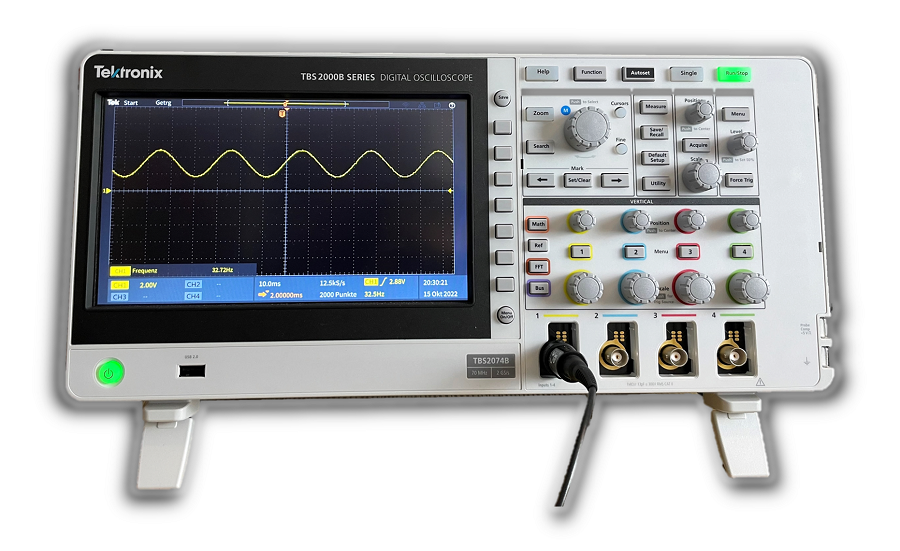
\includegraphics[width=\textwidth,height=6cm,keepaspectratio=true]{images/OszilloskopBeispiel.png}
%	\caption{
%		Oszilloskop aus \cite{OscilloscopeBild}
%	}
%	\label{Label}
%\end{figure} \newline
Komplexere Oszilloskope können häufig auch Messwerte persistent speichern oder die Skalierung der Achsen
ändern. Wegen letzterem lässt sich ein großer Umfang von Spannungswerten messen.
Durch diese Funktionen ist das Oszilloskop ein oft- und vielseitig verwendetes Messgerät
in der Elektrotechnik \cite{ETechnikEinfach}. \newline \newline
In dieser Seminararbeit wollen wir unser eigenes Oszilloskop bauen, das die Grundfunktionen,
eine Zeit lang Spannungen  zu messen und darzustellen, erfüllen soll.
Hierfür werden zuerst die groben Komponenten und deren Zusammenspiel im selbstgebauten Oszilloskop erläutert.\newline
Danach wird auf die einzelnen Bauteile und ihre Funktion eingegangen und
zuletzt eine Messung eines einfachen Schwingkreises durchgeführt, um an diesen Messwerten zu begründen,
ob das Oszilloskop die Anforderungen erfüllt.  

